\chapter{Gerêcia de requisitos}
Neste capítulo serão apresentados os requisitos elicitados, desde os épicos, localizados no mais alto nível do SAFe até as histórias de usuário no nível \textit{Team}, o nível mais abaixo no SAFe.

Para a gerência de requisitos, foi utilizada a ferramenta \textit{TargetProcess}, como foi proposto no trabalho 1.
\section{Portfolio}
O \textit{Portfolio} é o mais alto nível nível no SAFe, nesta etapa do trabalho o nível de portfólio é evidenciado pelas seguintes atividades: Analisar o contexto, Definir o tema de investimento, Elicitar e validar os épicos do negócio e priorizar um épicos. Atividades essas que foram realizadas utilizando algumas técnicas de elicitação como: Entrevistas, Workshops e Brainstorm.
\subsection{Requisitos elicitados}
\textbf{Tema de investimento} - Gestão de clientes da EletronJun

Este tema foi extraído a partir da necessidade de organização e gestão dos clientes da empresa, visando facilitar a comunicação, além de aumentar a produtividade e a organização da empresa.

\textbf{Épico 01} - Gerenciamento de clientes

Compreente todas as ações do cliente dentro do sistema.

\textbf{Épico 02} - Gerenciamento de pedidos

Contém um registro de todos os pedidos realizados pelo cliente.

\textbf{Épico 03} - Gerenciamento de pagamentos

Contém um registro de todos os pagamentos do cliente.

\textbf{Épico 04} - Centralização da comunicação

Engloba toda a comunicação existente entre o cliente e a empresa.

A seguir os épicos estão sendo detalhados através do template \textit{lightwaight business case}, que é mencionado no \ref{safe}.

\begin{table}[]
\centering
\label{label-epico01}
\begin{tabular}{
>{\columncolor[HTML]{96FFFB}}r l}
\multicolumn{2}{c}{\cellcolor[HTML]{34CDF9}Gerenciamento de clientes} \\
Para          & A empresa e seus clientes \\
Quem          & Faz a gestão dos clientes da empresa \\
A             & Sistema de gerenciamento de clientes \\
É uma         & Ferramenta que faz a gestão dos clientes da empresa dentro do sistema \\
Que           & Centraliza e facilita a gestão dos clientes em uma só ferramenta, aumentando a organização e a produtividade da empresa \\
Diferente     & Da forma como é feita atualmente, onde não há um gerenciamento eficiente e a rastreabilidade dos clientes é nula \\
Nossa solução & Um sistema único e modularizado, onde existirá o módulo de gestão de clientes da EletronJun \\
\multicolumn{2}{c}{\cellcolor[HTML]{34CDF9}Escopo} \\
Critérios de sucesso & Implementação de um único sistema para a gestão de clientes de forma que a organização aumente e consequentemente a produtividade da empresa \\
No escopo            & Sistema para a gestão dos clientes \\
Fora do escopo       & Aprovação do sistema pelos clientes 
\end{tabular}
\caption{Épico 01}
\end{table}

\begin{table}[]
\centering
\label{label-epico02}
\begin{tabular}{
>{\columncolor[HTML]{96FFFB}}r l}
\multicolumn{2}{c}{\cellcolor[HTML]{34CDF9}Gerenciamento de pedidos}            \\
Para                 & A empresa e seus clientes                       \\
Quem                 & Faz a gestão dos pedidos realizados pelos clientes da empresa            \\
A                    & Sistema de gerenciamento de pedidos             \\
É uma                & Ferramenta que faz a gestão dos pedidos realizados pelos clientes                      \\
Que                  & Melhora a forma como os pedidos são feitos, centralizando-os em uma única ferramenta                     \\
Diferente            & Da forma como é feita atualmente, onde não há um gerenciamento eficiente e não é feito nenhum registro dos pedidos para uma consulta posterior                       \\
Nossa solução        & Um sistema único e modularizado, onde existirá o módulo de gestão de pedidos realizados pelos clientes da EletronJun          \\
\multicolumn{2}{c}{\cellcolor[HTML]{34CDF9}Escopo}                     \\
Critérios de sucesso & Implementação de um único sistema para a gestão de pedidos realizados pelos clientes de forma que a organização aumente e consequentemente a produtividade da empresa \\
No escopo            & Sistema para a gestão de pedidos realizados pelos clientes   \\
Fora do escopo       & Aprovação do sistema pelos clientes            
\end{tabular}
\caption{Épico 02}
\end{table}

\begin{table}[]
\centering
\label{label-epico03}
\begin{tabular}{
>{\columncolor[HTML]{96FFFB}}r l}
\multicolumn{2}{c}{\cellcolor[HTML]{34CDF9}Gerenciamento de pagamentos}   \\
Para                 & A empresa e seus clientes              \\
Quem                 & Faz a gestão dos pagamentos realizados pelos clientes da empresa              \\
A                    & Sistema de pagamentos                  \\
É uma                & Ferramenta que faz a gestão dos pagamentos realizados pelos clientes          \\
Que                  & Centraliza e facilita os pagamentos realizados pelos clientes, aumentando a organização e os lucros da empresa       \\
Diferente            & Da forma como é feita atualmente, onde o cliente envia um email para a empresa e a empresa envia um número de conta bancária para que o cliente faça um depósito         \\
Nossa solução        & Um sistema único e modularizado, onde existirá o módulo de pagamentos realizados pelos clientes da EletronJun, visando disponibilizar mais opções de pagamento para o cliente, como cartão de crédito, boleto e PagSeguro, além de permitir uma gestão dos pagamentos realizados \\
\multicolumn{2}{c}{\cellcolor[HTML]{34CDF9}Escopo}            \\
Critérios de sucesso & Implementação de um único sistema para o pagamento dos pedidos realizados pelos clientes de forma que aumente a organização e consequentemente os lucros da empresa       \\
No escopo            & Sistema para o pagamento de pedidos realizados pelos clientes                 \\
Fora do escopo       & Aprovação do sistema pelos clientes   
\end{tabular}
\caption{Épico 03}
\end{table}

\begin{table}[]
\centering
\label{label-epico04}
\begin{tabular}{
>{\columncolor[HTML]{96FFFB}}r l}
\multicolumn{2}{c}{\cellcolor[HTML]{34CDF9}Centralização da comunicação}  \\
Para                 & A empresa e seus clientes\\
Quem                 & Faz a comunicação cliente/empresa     \\
A                    & Sistema para a comunicação            \\
A                    & Sistema para a comunicação            \\
É uma                & Ferramenta que facilita a comunicação entre a empresa e o cliente            \\
Que                  & Centraliza a comunicação cliente/empresa em uma única ferramenta aumentando assim a rastreabilidade e a organização \\
Diferente            & Da forma como é feita atualmente, onde a comunicação é feita por diversos meios diferentes e não há uma rastreabilidade da comunicação feita  \\
Nossa solução        & Um sistema único e modularizado, onde existirá um módulo para a comunicação entre o cliente e a empresa\\
\multicolumn{2}{c}{\cellcolor[HTML]{34CDF9}Escopo}           \\
Critérios de sucesso & Implementação de um único sistema para a comunicação cliente/empresa de forma que aumente a organização e consequentemente a produtividade da empresa \\
No escopo            & Sistema para comunicação cliente/empresa                        \\
Fora do escopo       & Aprovação do sistema pelos clientes  
\end{tabular}
\caption{Épico 04}
\end{table}
\section{Program}
O \textit{Program} é o nível intermediário no SAFe, nesta etapa do trabalho o nível de programa é evidenciado pelas seguintes atividades: Elicitar \textit{features} e requisitos não-funcionais, definir o Visão(presente nos anexos) e priorizar uma \textit{feature}.
\subsection{Requisitos elicitados}
\textbf{\textit{Feature 01}} - Manutenção de clientes

\textbf{\textit{Feature 02}} - Manutenção de pedidos

\textbf{\textit{Feature 03}} - Meios de pagamento

\textbf{\textit{Feature 04}} - Registro de pagamentos

\textbf{\textit{Feature 05}} - Manutenção da comunicação
\subsection{Requisitos não-funcionais}
\subsection{Visão}
O documento de visão produzido está localizado no Anexo B.
\subsection{Roadmap}
O \textit{roadmap} funciona como um documento que faz a padronização entre o nível de time e programa, é um "caminho" a ser seguido no cronograma das entregas planejadas. Representa os incrementos do software que devem ser entregues. Existem dois tipos de \textit{roadmap}: \ref{safe}
\begin{itemize}
\item \textbf{síncrono}: \textit{features} são entregues sincronizadas, em cada \textit{release} é entregue uma \textit{feature}.
\item \textbf{assíncrono}: \textit{features} são entregues por versões, uma \textit{release} não precisa conter uma \textit{feature} completa, mas sim uma versão que pode ser incrementada, na próxima \textit{release}.
\end{itemize}

O nosso planejamento foi baseado no \textit{roadmap} síncrono, ilustrado na imagem abaixo:
  \begin{figure}[!htbp]
    \centering
    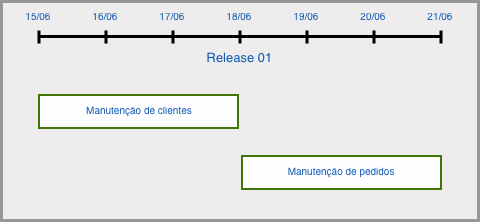
\includegraphics[scale=0.75]{figuras/roadmap}
    \caption[Roadmap]{Roadmap\footnotemark}
    \label{Roadmap}
  \end{figure}
  
\section{Team}
O \textit{Team} é o último nível do SAFe, nesta etapa do trabalho o nível de time é evidenciado pelas seguintes atividades: Elicitar e Validar histórias de usuário, Planejar \textit{Sprint}, Exexutar e Gerenciar \textit{Sprint}, e fazer a Retrospectiva e a Revisão da \textit{Sprint}.
\subsection{Requisitos elicitados}
\textbf{\textit{História de usuário 01}} - Eu como cliente gostaria de um sistema no qual eu pudesse ter uma conta pessoal. Para que assim eu possa gerenciar os meus acessos e as minhas atividades.

\textbf{\textit{História de usuário 02}} - Eu como cliente, gostaria de gerenciar a minha conta. Para que eu possa manter a minha conta da melhor forma pelo tempo que for necessário.

\textbf{\textit{História de usuário 03}} - Eu como cliente, gostaria de um sistema no qual eu pudesse fazer um orçamento dos projetos. Para que eu possa ter uma ideia do custo do projeto antes de fazer o pedido.

\textbf{\textit{História de usuário 04}} - Eu como cliente, gostaria de um sistema no qual eu pudesse fazer pedidos. Para que eu envie os projetos e faça os pedidos.

\textbf{\textit{História de usuário 05}} - Eu como cliente, gostaria de um sistema no qual eu pudesse gerenciar os pedidos realizados. Para que seja mantido um histórico possibilitando um controle melhor de todos os pedidos.

\textbf{\textit{História de usuário 06}} - Eu como cliente, gostaria de um sistema no qual eu pudesse acompanhar o status de um pedido. Para que eu possa saber em que fazer de desenvolvimento está o projeto do qual eu fiz o pedido.

\textbf{\textit{História de usuário 07}} - Eu como cliente, gostaria de um sistema no qual eu pudesse efetuar pagamentos por diferentes meios. Para que eu tenha mais opções na hora de efetuar o pagamento pelo meu projeto.

\textbf{\textit{História de usuário 08}} - Eu como empresa/cliente, gostaria de um sistema no qual eu pudesse gerenciar os pagamentos realizados. Para que assim eu possa manter um histórico e um controle melhor da parte financeira.

\textbf{\textit{História de usuário 09}} - Eu como cliente, gostaria de um sistema no qual eu pudesse ter um canal de comunicação entre a empresa/cliente. Para que a comunicação seja mais fácil e centralizada em um local.

\section{Gerência de mudança}
\subsection{Atributos de requisitos}
Os atributos contém as informações mais importantes daquele requisito, são suas propriedades, e é a partir dessas propriedades que se tem informações como: data de criação, origem, importância, dentre outras. Demandam atenção durante a sua especificação, pois fornecem importantes informações sobre o estado do projeto, além de permitirem que sejam realizadas consultas dentro de todos os requisitos.
\begin{itemize}
\item \textbf{Prioridade} - Indica o quão importante o requisitos é para os \textit{stakeholders} e/ou para o sistema.
\item \textbf{Complexidade} - Indica a quantidade de esforço que um determinado requisito irá demandar, o quão difícil é a sua implementação. Também pode ser utilizado para medir o tempo que o requisito levará para ser finalizado.
\item \textbf{Responsável} - Define qual membro da equipe é responsável por aquele requisito naquele momento. Pode ser alterado durante a execução do projeto.
\item \textbf{Status} - Indica o grau de completude do requisito.
\end{itemize}
\subsection{Rastreabilidade de requisitos}
Rastreabilidade de software é a habilidade de relacionar artefatos criados durante o ciclo de vida de desenvolvimento de um sistema de software. Os elementos rastreáveis do projeto são chamados de itens de rastreabilidade.

As necessidades de rastreabilidade das diferentes partes interessadas, como: patrocinadores, gerentes, analistas, designers, mantenedores e usuários, diferem devido a mudanças em seus objetivos e prioridades. A rastreabilidade de requisitos é uma característica do sistema em que os requisitos estão claramente ligados às suas fontes, e os artefatos criados durante o ciclo de vida do desenvolvimento de sistemas com base nesses requisitos.

O rastreamento de requisitos pode ser visto como uma habilidade de acompanhar e descrever a vida de um requisito em abas as direções. A pré-rastreabilidade documenta o contexto a partir do qual emergem os requisitos, já a pós-rastreabilidade vincula os requisitos ao desenho do sistema e sua implementação~\cite{davis}.

\begin{figure}[!htbp]
\centering
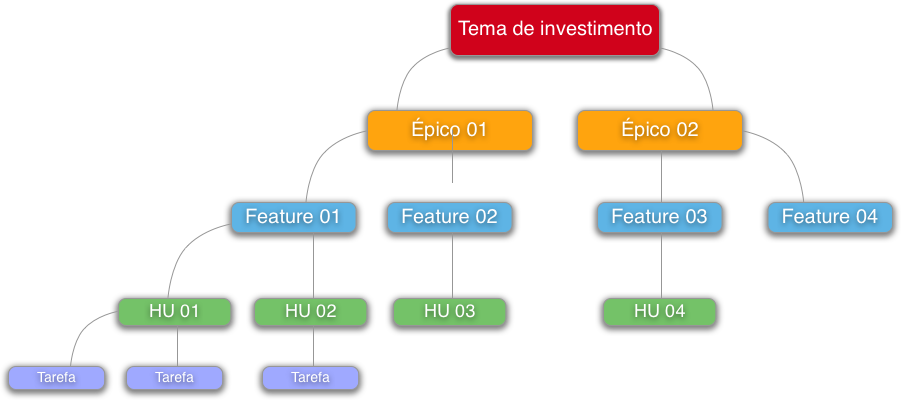
\includegraphics[scale=0.45]{figuras/matriz_rastreabilidade}
\caption[Visão geral da rastreabilidade]{Visão geral da rastreabilidade\footnotemark}
\label{Rastreabilidade}
\end{figure}

A ferramenta de gerenciamento de requisitos utilizada é a \textit{TargetProcess}. As figuras~\ref{targetprocess_ep1}, \ref{targetprocess_ep2}, \ref{targetprocess_ep3} e \ref{targetprocess_ep4} mostram os épicos registrados e como a ferramenta trata a rastreabilidade vertical do sistema.

\begin{figure}[!htbp]
\centering
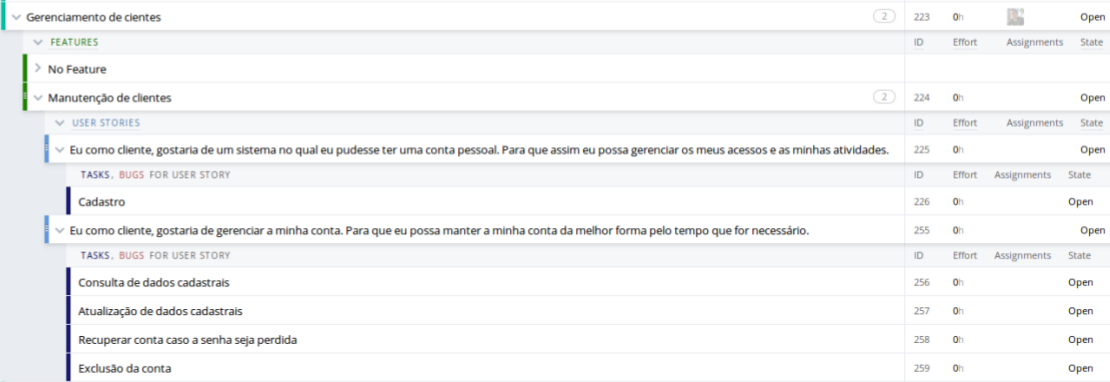
\includegraphics[width=0.75\textwidth]{figuras/targetprocess_ep1}
\caption{Rastreabilidade vertical da ferramenta: épico 1.}
\label{targetprocess_ep1}
\end{figure}

\begin{figure}[!htbp]
\centering
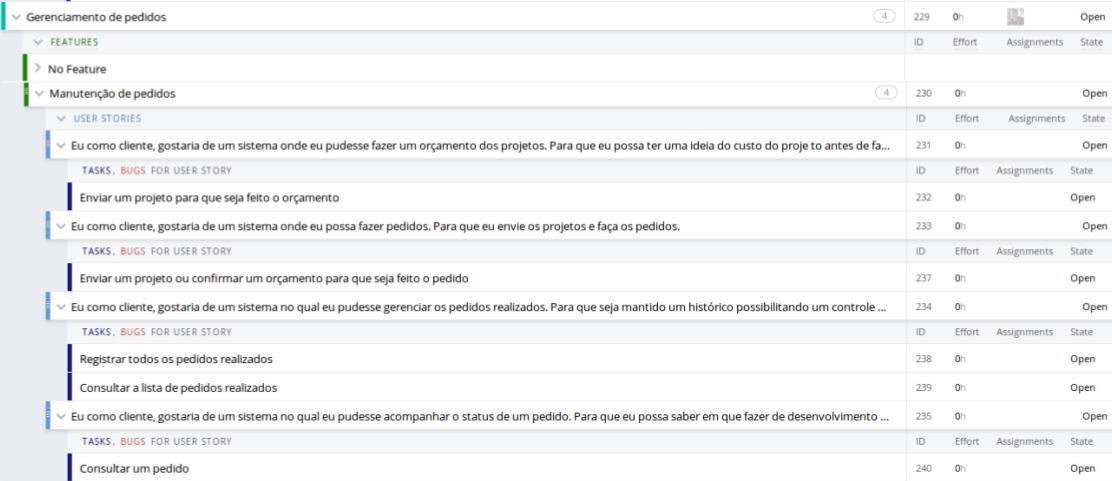
\includegraphics[width=0.75\textwidth]{figuras/targetprocess_ep2}
\caption{Rastreabilidade vertical da ferramenta: épico 2.}
\label{targetprocess_ep2}
\end{figure}

\begin{figure}[!htbp]
\centering
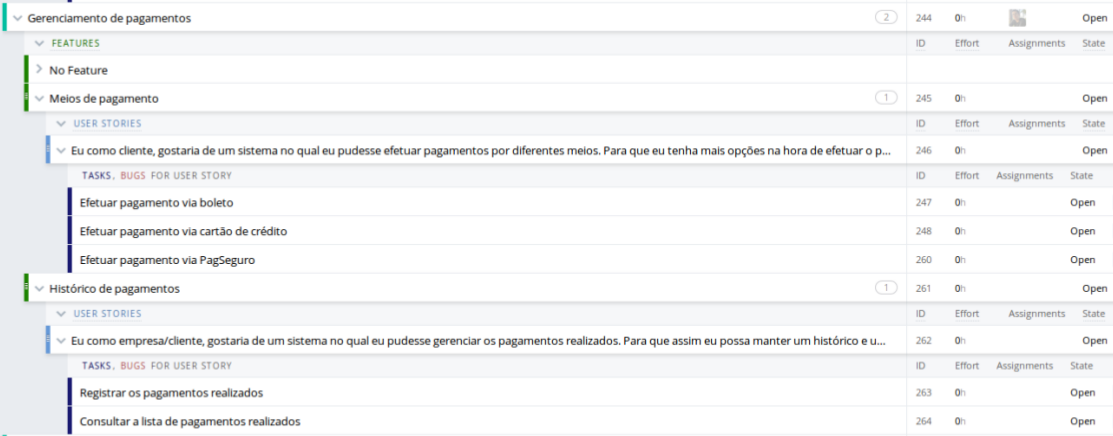
\includegraphics[width=0.75\textwidth]{figuras/targetprocess_ep3}
\caption{Rastreabilidade vertical da ferramenta: épico 3.}
\label{targetprocess_ep3}
\end{figure}

\begin{figure}[!htbp]
\centering
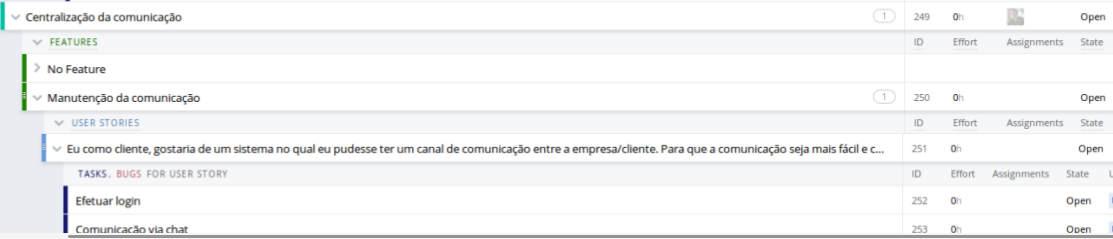
\includegraphics[width=0.75\textwidth]{figuras/targetprocess_ep4}
\caption{Rastreabilidade vertical da ferramenta: épico 4.}
\label{targetprocess_ep4}
\end{figure}

